% !TEX root = ../main.tex


\section{Run To Completion}

The run to completetion sematics is implemented via a basis that is extend by the model. 
Figure~\ref{fig:basis} shows a statechart representation of how the basis enforces 
the run to completion semantics on the model transitions.
\begin{figure}[!h]
	\vspace{-.4cm}
	\centering
	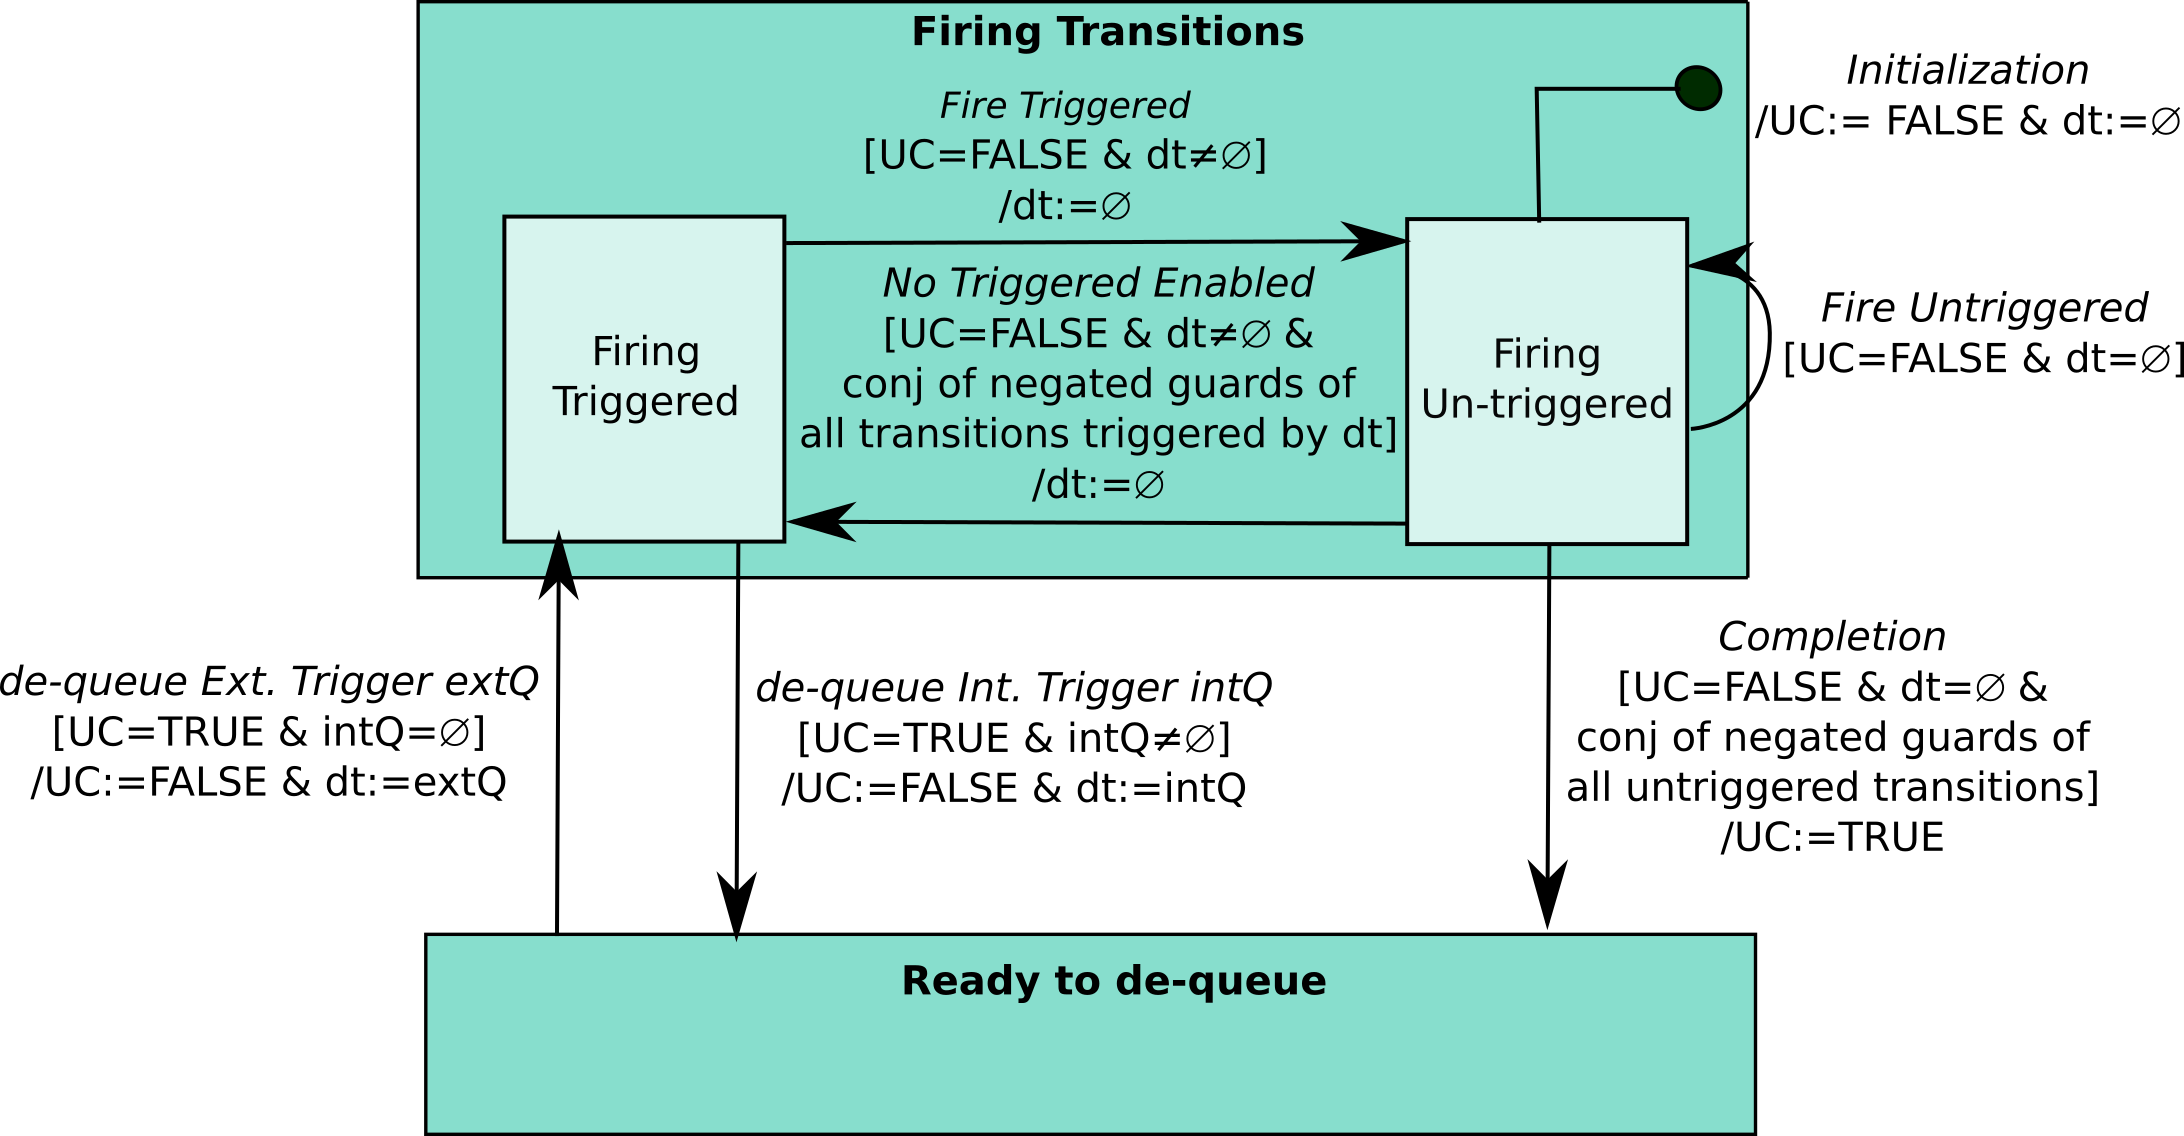
\includegraphics[width=0.99\textwidth]{figures/basis.png}
	\caption{Abstract representation of run to completion basis}
	\label{fig:basis}
	\vspace{-.4cm}
\end{figure}

The translation from \SCXML to \EVENTB is based on an abstract `basis' that models the `run to completion' semantics. 
This basis consists of an \EVENTB \emph{context} and \emph{machine} that are the same for all input models and are refined by the specific output of the translation.  
The basis context, Listing~\ref{lst:BasisContext}, introduces a given set of all possible triggers that is partitioned into internal and external ones, some of which will be introduced in future refinements. 
Refinements partition these trigger sets further to introduce concrete triggers, leaving a new abstract set to represent the remaining triggers yet to be introduced. 

For example, the IDS model introduces a specific internal trigger, \textbf{spi\_done},  by partitioning |SCXML_FutureInternalTrigger| into the singleton \textbf{\{spi\_done\}} and a new set, |SCXML_FutureInternalTrigger0|, representing the remainder. 
 % as shown in line~\ref{line:refPartition} of Listing~\ref{lst:SecBotCont0}. 

\begin{lstlisting}[caption={Abstract basis context},label={lst:BasisContext}, language=Event-B, escapechar=|, frame=single, basicstyle=\rmfamily\scriptsize, belowskip=-2.0 \baselineskip, float=t]
context
	basis_c 	// (generated for SCXML)
sets
	SCXML_TRIGGER	 // all possible triggers
constants
	SCXML_FutureInternalTrigger	 // all possible internal triggers
	SCXML_FutureExternalTrigger	 // all possible external triggers  
axioms
	partition(SCXML_TRIGGER, SCXML_FutureInternalTrigger, SCXML_FutureExternalTrigger) 
end
\end{lstlisting}	

% \begin{lstlisting}[caption={Context for \IDS abstract model},label={lst:SecBotCont0}, language=Event-B, escapechar=|, frame=single]
% context
% 	IDS_Model_0_ctx //(generated from:/IDS_generated/secbot.scxml)
% extends
% 	basis_c 
% constants
% 	SCXML_FutureInternalTrigger0	
% 	SCXML_FutureExternalTrigger0
% 	spi_done	 	//trigger
% axioms
% 	SCXML_FutureExternalTrigger0=SCXML_FutureExternalTrigger
% 	partition(SCXML_FutureInternalTrigger, SCXML_FutureInternalTrigger0,{spi_done}) |\label{line:refPartition}|
% end
% \end{lstlisting}

The basis machine, part of which is shown in Listing~\ref{lst:BasisMachine}, declares variables that correspond to the triggers present in the queue at any given time, and a flag, |SCXML_uc|, that signals when a run to completion macro-step has been completed (no un-triggered transitions are enabled). 
After initialisation, both trigger queues are empty and |SCXML_uc| is set to |FALSE| so that un-triggered transitions are dealt with. 
The basis machine provides events that describe the generic behaviour of models that follow the run to completion semantics in terms of altering the trigger queues and completion flag.
Since new events introduced in a refinement cannot modify existing variables, all future events generated by translation of the specific \SCXML model, will refine these abstract events.
The abstract event, |SCXML_futureExternalTrigger| represents the raising of an external trigger.    
The abstract event, |SCXML_futureInternalTransitionSet| represents a combination of transitions that are triggered by an internal trigger. 
The guards of this event ensure prior completion of the previous macro-step. 
A similar event, |SCXML_futureExternalTransitionSet| (not shown) represents a combination of transitions that are triggered by an external trigger and has the additional guard that the internal trigger queue is empty.
These two triggered transition events reset the completion flag to ensure that any un-triggered transitions that may have become enabled have a chance to fire next.
The abstract event |SCXML_futureUntriggeredTransitionSet| represents a combination of transitions that are un-triggered and may only be fired when the completion flag is unset (FALSE).
It leaves the completion flag unset in case further combinations of un-triggered transitions are enabled.
All three of these transition events also allow for raising a non-deterministic set of internal triggers.
A final abstract event, |SCXML_completion|, sets the completion flag (TRUE) if it is not already set. At this abstract basis level, this is non-deterministically fired since we do not yet have any detail of what needs to be completed.

\begin{lstfloat}[!tb]
\begin{lstlisting}[caption={Abstract basis machine (part of)}, label={lst:BasisMachine},language=Event-B, escapechar=|, frame=single, basicstyle=\rmfamily\scriptsize, belowskip=-2.0 \baselineskip]
machine basis_m  sees basis_c // (generated for SCXML)
variables
	SCXML_iq	  // internal trigger queue
	SCXML_eq	  // external trigger queue
	SCXML_uc	  // run to completion flag
invariants
	SCXML_iq ⊆ SCXML_FutureInternalTrigger	// internal trigger queue
	SCXML_eq ⊆ SCXML_FutureExternalTrigger	// external trigger queue
	SCXML_iq ∩ SCXML_eq= ∅					// queues are disjoint
	SCXML_uc ∈ BOOL							// completion flag
events

	INITIALISATION: 
	begin
		SCXML_iq := {}		//internal Q is initially empty
		SCXML_eq := {}		//external Q is initially empty
		SCXML_uc := FALSE	//completion is initially FALSE
	end

	SCXML_futureExternalTrigger: 
	any SCXML_raisedTriggers where
		SCXML_raisedTriggers ⊆ SCXML_FutureExternalTrigger 
	then
		SCXML_eq ≔ SCXML_eq ∪ SCXML_raisedTriggers 
	end

	SCXML_futureInternalTransitionSet: 
	any SCXML_it SCXML_raisedTriggers where
		SCXML_it ∈ SCXML_iq 
		SCXML_uc = TRUE 
		SCXML_raisedTriggers ⊆ SCXML_FutureInternalTrigger 
	then
		SCXML_uc ≔ FALSE 
		SCXML_iq ≔ (SCXML_iq ∪ SCXML_raisedTriggers) ∖ {SCXML_it} 
	end

	SCXML_futureUntriggeredTransitionSet: 
	any SCXML_raisedTriggers where
		SCXML_uc = FALSE
		SCXML_raisedTriggers ⊆ SCXML_FutureInternalTrigger
	then
		SCXML_uc ≔ FALSE 
		SCXML_iq ≔ SCXML_iq ∪ SCXML_raisedTriggers 
	end

end
\end{lstlisting}
\end{lstfloat}

\begin{lstfloat}[!tb]
\begin{lstlisting}[caption={Event-B event corresponding to internal triggered transition to \textbf{Wait50ms} state in refinement level 1 shown in Fig.~\ref{fig:ASIC}}, label={lst:SecBotMach0},language=Event-B, escapechar=|, frame=single, belowskip=-2.0 \baselineskip]
spi_done__InitialiseSensor_Wait50ms:	
refines SCXML_futureInternalTransitionSet 
any SCXML_it SCXML_raisedTriggers where
SCXML_it  ∈ SCXML_iq 
SCXML_uc = TRUE
SCXML_raisedTriggers ⊆ SCXML_FutureInternalTrigger
InitialiseSensor = TRUE
SCXML_it = spi_done  	//trigger for this transition |\label{line:defTrigger}|
then
SCXML_uc ≔ FALSE
SCXML_iq ≔ (SCXML_iq ∪ SCXML_raisedTriggers) ∖ {SCXML_it}
InitialiseSensor ≔ FALSE
Wait50ms ≔ TRUE
end
\end{lstlisting}
\end{lstfloat}